\documentclass[12pt, a4paper]{article}
\usepackage{enumitem}
\setlist[enumerate]{label = (\roman*)}
\usepackage{amsmath}
\usepackage{mathtools}
\usepackage{amssymb}
\usepackage{amsthm}
\theoremstyle{definition}
\newtheorem{example}{Example}

\usepackage{tikz}
\usepackage{hyperref}

\newcommand{\summation}[2]{\sum\limits_{#1}^{#2}}
\newcommand{\limit}[2]{\lim\limits_{#1\to #2}}
\newcommand{\vep}{\varepsilon}


\begin{document}
\begin{example}[CES utility function]
The constant elasticity of substitute utility function has form of,
\[
U(x) = (\summation{i=1}{n} x_i^{\rho})^{\frac{1}{\rho}}.
\]
The constant elasticity is indeed: $\frac{1}{1-\rho}$, before we proceed to proof notice that 
\[
MRS_{ji} = \frac{\frac{1}{\rho}(\sum\limits_{i=1}^n x_i^{\rho})^{\frac{1-\rho}{\rho}}\rho x_j^{\rho-1}}{\frac{1}{\rho}(\sum\limits_{i=1}^n x_i^{\rho})^{\frac{1-\rho}{\rho}}\rho x_i^{\rho-1}}=(\frac{x_j}{x_i})^{\rho -1}
\]
Hence,
\begin{align*}
E_{ij} &= \frac{\partial ln(\frac{x_i}{x_j})}{\partial ln(MRS_{ji})}\\
&=\frac{\partial ln(\frac{x_i}{x_j})}{\partial ln[({\frac{x_i}{x_j})}^{1-\rho}]}\\
&=\frac{1}{1-\rho}.
\end{align*}
\end{example}

\begin{example}[CES production function]
The CES production function is given by, 
\[
f(x)=A(\summation{i=1}{n}\lambda_ix_i^{\rho})^{\frac{k}{\rho}}.
\]
More often, we focus on $f(x)=(\summation{i=1}{n}a_ix_i^{\gamma})^{\frac{1}{\gamma}}$ with $\summation{i=1}{n}a_i=1$ and this form has following three ``transformations" according to different cases of $\gamma s$.
\begin{enumerate}
\item $\limit{r}{1}(\summation{i=1}{n}a_ix_i^{\gamma})^{\frac{1}{\gamma}} = \summation{i=1}{n}a_ix_i$: this is obvious;
\item $\limit{r}{0} (\summation{i=1}{n}a_ix_i^{\gamma})^{\frac{1}{\gamma}} = \prod\limits_{i=1}^n x_i^{a_i}$: 
\begin{proof}
\[
\limit{r}{0} (\summation{i=1}{n}a_ix_i^{\gamma})^{\frac{1}{\gamma}}= \limit{r}{0}e^{\frac{1}{\gamma}ln(\sum\limits_{i=1}^n a_ix_i^{\gamma})}
\]
Notice that L'H\^opital's Rule implies,
\[
\limit{r}{0}\frac{ln(\summation{i=1}{n}a_ix_i^{\gamma})}{\gamma}\to
\]

\[
e^{\summation{i=1}{n}a_iln(x_i)}=\prod\limits_{i=1}^nx_i^{a_i}.
\]
\end{proof}
\end{enumerate}
\end{example}

\begin{example}[Shadow price]
Lagrange multipliers is interpreted as the change in the objective function by relaxing the constraint by one unit, in economics that change can be seen as a value or "shadow price". We shall prove this. 
    
The formal idea is below: say, you are facing the following constrained optimization problem:

\[
\begin{dcases}
\max_{(x,y)} &{}f(x,y) \\
\textrm{s.t.} &{}g(x,y)=c
\end{dcases}\longrightarrow
\begin{dcases}
x^{*} &= x^{*}(c)\\
y^{*} &= y^{*}(c)\\
\lambda^{*} &= \lambda^{*}(c)
\end{dcases}
\]

We briefly sketch the process of Lagrangian method:
\begin{enumerate}
\item Construct the Lagrangian equation: $\mathcal{L}(x,y,\lambda) = f(x,y)+\lambda(c-g(x,y))$
\item Take the derivative with regard to $x,y,\lambda$, then we get the first order condition:
\begin{align*}
\frac{\partial \mathcal{L}(x^{*},y^{*},\lambda^{*})}{\partial x}&=\frac{\partial f(x^{*},y^{*})}{\partial x}-\lambda^{*}\frac{\partial g(x^{*},y^{*})}{\partial x}=0\\
\frac{\partial \mathcal{L}(x^{*},y^{*},\lambda^{*})}{\partial y}&=\frac{\partial f(x^{*},y^{*})}{\partial y}-\lambda^{*}\frac{\partial g(x^{*},y^{*})}{\partial y}=0\\
\frac{\partial \mathcal{L}(x^{*},y^{*},\lambda^{*})}{\partial \lambda}&=c-g(x^{*},y^{*})=0
\end{align*}
\item Solve this system equations and get the results.
\end{enumerate}

Now, you may wonder if we increase $c$ by one unit, how much would $f(x^{*},y^{*})$ increase? The answer is: $\lambda^{*}$, that's why Lagrange multipliers are called \emph{shadow prices}, i.e., the change in the objective function by relaxing the constraint by one unit. Let's prove it.
\begin{proof}
Writing the value function as: $F(c) = f(x^{*}(c),y^{*}(c))$, now take derivative with respect to $c$:
\begin{align*}
\frac{dF(c)}{dc} &= \frac{\partial f(x^{*}(c),y^{*}(c))}{\partial x}\cdot \frac{dx^{*}(c)}{dc}+\frac{\partial f(x^{*}(c),y^{*}(c))}{\partial y}\cdot \frac{dy^{*}(c)}{dc}\\
&=\underbrace{\lambda^{*}(c)\cdot \frac{\partial g(x^{*},y^{*})}{\partial x}}_{FOC}\cdot \frac{dx^{*}(c)}{dc}+\underbrace{\lambda^{*}(c)\cdot\frac{\partial g(x^{*},y^{*})}{\partial y}}_{FOC}\cdot \frac{dy^{*}(c)}{dc}\\
&=\lambda^{*}(c)\cdot\underbrace{(\frac{\partial g(x^{*},y^{*})}{\partial x}\cdot \frac{dx^{*}(c)}{dc}+\frac{\partial g(x^{*},y^{*})}{\partial y}\cdot \frac{dy^{*}(c)}{dc})}_{\textrm{Take differential with }c:\;g(x,y)=c\implies 1}\\
&=\lambda^{*}(c)
\end{align*}
Analogize to the utility maximizing problem, the interpretation of Lagrange multiplier is: when you have one unit more wealth, then your total utility would increase by $\lambda^{*}$.
\end{proof}
\end{example}

\begin{example}[Binary relation as a subset of Cartesian product]
Consider outcome set $X=\{a,b,c\}$, we can define a binary relation 
\[
\succsim = \{(a,a),(b,b),(c,c),(a,b),(b,a),(a,c),(b,c)\}.
\] 
\end{example}

\begin{example}[Continuous preference with discontinuous utility function]
A continuous preference can be represented by a discontinuous utility function. Consider $X=\mathbb{R}$ and $\succsim$ is ``more is better". Clearly $\succsim$ is continuous, however it can be represented as
\[
U(x)=\begin{dcases}
x, &\text{ if }x\leq 0,\\
x+1, &\text{ if }x>0. 
\end{dcases}
\]
\end{example}

\begin{example}[Implication of local-nonsatiation preference]
Consider two bundles $x^j$ and $x^k$. $x^j= (x_1^j,x_2^j,\dots,x_n^j)$ and $x^k=(x_1^k,x_2^k,\dots,x_n^k)\in \mathbb{R}_+^n$. Bundle $x^j$ satisfies this: when facing price vector $p^j=(p_1^j,p_2^j,\dots,p_n^j)$, the consumer chooses $x^j$. Bundle $x^k$ is affordable under $p^j$, i.e., $p^jx^k<p^jx^j$. 

\emph{Claim}: If the decision maker's choices can be rationalized by a complete locally non-satiated preference relation, then it must be the case that $x^j\succ x^k$.
\begin{proof}
We will prove it by contradiction. Assume: $x^k\succsim x^j$ and consider 
\[
\vep = \frac{p^jx^j-p^jx^k}{\summation{i=1}{n} p^j_i}.
\]
\begin{align*}
&\implies \summation{i=1}{n}p_i^jy_i <\summation{i=1}{n}p_i^j(x_i^k+\vep),\;\forall y \in B_{\vep}(x_k)\\
&\implies \summation{i=1}{n}p_i^jy_i<\summation{i=1}{n}p_i^jx_i^k+\vep\summation{i=1}{n}p_i^j \\
&\implies \summation{i=1}{n}p_i^jy_i<\summation{i=1}{n}p_i^jx_i^k+\frac{p^jx^j-p^jx^k}{\summation{i=1}{n} p_i^j}\summation{i=1}{n}p^j_i\\
&\implies p^jy<p^jx^j
\end{align*}

This means that you find a ball around $x^k$, such that at price $p^j$, every $y \in B_{\vep}(x^k)$ is affordable.

By non-satiation assumption, $\exists y'\in B_\vep(x^k)$, such that $y'\succ x^k\succsim x^j$. This leads to the contradiction that $\succsim$ rationalized choices, since at price $p^j$ bundle $x^j$ is optimal for decision maker.
\end{proof}
\end{example}

\begin{example}[Convex preference may not have concave utility representation]
Let's consider the preference on $\mathbb{R}$ such that $x\succsim y$ if $x\geq y$ or $y<0$. This preference is convex but does not have concave utility representation.
\begin{proof}
First we prove it's convex then we show it does not have concave utility function.
\begin{enumerate}
\item \emph{The preference is convex: }we want to show $AsGoodAs(y)=\{z|z\succsim y\}$ for any $y$ in $\mathbb{R}$ is convex. $y$ has the following two cases.
\begin{enumerate}
\item $y\geq 0$: $\forall x,z\succsim y$ and $\alpha\in (0,1)$, we have $\alpha x + (1-\alpha)z \geq y$. This implies $\alpha x + (1-\alpha)z\succsim y\implies (\alpha x +(1-\alpha)z)\in AsGoodAs(y)$.
\item $y<0$. Then $x,z$ have the following three cases.
\begin{enumerate}
\item $x,z\geq 0$: $\alpha x+(1-\alpha)z\geq 0> y$. This implies $(\alpha x +(1-\alpha)z) \in AsgoodAs(y)$
\item $x\geq 0$ and $z<0$: $\alpha x + (1-\alpha)z$ is either $\geq 0$ or $<0$, both cases imply $\alpha x + (1-\alpha)z \in AsGoodAs(y)$.
\item $x<0$ and $z<0$: $\alpha x + (1-\alpha)z \sim y$, therefore $\alpha x + (1-\alpha)z\in AsGoodAs(y)$. 
\end{enumerate}
\end{enumerate} 
\item \emph{The utility representation is not concave: }$\{x<0\}$ is mapped into a flat line and $\{x\geq0\}$ is mapped into an increasing function, therefore it can not be concave.
\end{enumerate}
\end{proof}
\end{example}

\begin{example}[Monotonic preference does not imply non-giffen good]
Consider the following utility function with two commodities:
\[
u(x) = \min\{u_1(x), u_2(x) \},\text{ where }u_1(x) = x_1 + 10,\;u_2(x) = 2(x_1+x_2)
\]
Now consider the following case, consumer's income is $m=60$, $p_1 = 12$ and $p_2$ changes from $9$ to $4$. \begin{figure}[h!]
\centering
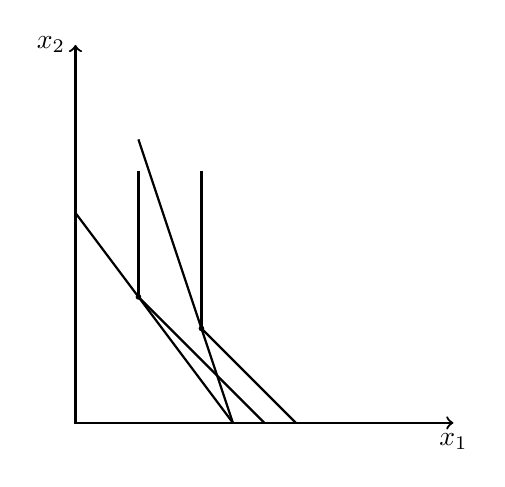
\begin{tikzpicture}[scale = 0.4]
\draw [<->, thick] (0,12) node [left] {$x_2$} -- (0,0) -- (12,0) node [below] {$x_1$};
\draw [thick] (0,20/3) -- (5,0);
\draw [thick] (2,8) -- (2,4);
\draw [thick] (2,4) -- (6,0);
\filldraw [fill = black] (2,4) circle (2pt);
\draw [thick] (2,9) -- (5,0);
\draw [thick] (4,8) -- (4,3);
\draw [thick] (4,3) -- (7,0);
\filldraw [fill = black] (4,3) circle (2pt);
\end{tikzpicture}
\caption{Good $2$ is Giffen good}
\end{figure}
This graph shows that when price of good $2$ decreases, however, consumer's demand for good $2$ decreases as well! Meanwhile, consumer's preferences are \emph{monotonic}!
\end{example}

\begin{example}[Turtle traveling]
Consider the following two sentences:
\begin{enumerate}
\item The maximal distance a turtle can travel in $2$ days is $7$ km.
\item The minimal time it takes a turtle to travel $7$ km is $2$ days.
\end{enumerate}
under which conditions are these two sentences equivalent?
\begin{enumerate}
\item For $1$ implies $2$: we need \emph{monotonicity} of distance-day function. For example, consider the following distance-day function: a turtle can travel $7$ km in $1$ day but after $1$ day it has to rest. Then, this distance-day function is not monotonic and it does not imply $2$.
\item For $2$ implies $1$: we need \emph{continuity} of distance-day function. For example, consider a turtle can jump at $t=2$ from $d=7$ to $d=9$, then $1$ fails.
\end{enumerate}
Refer to figure \ref{fig2} for descriptive result.
\begin{figure}[h!]
\centering
\begin{tikzpicture}
\draw [<->] (0,4) node [above] {distances}-- (0,0) --(4,0) node [below] {days};
\draw [thick] (0,0) -- (1.5,3) -- (3,3);
\draw [dashed] (1.5,3) -- (0,3) node [left] {$7$};
\draw [dashed] (1.5,3) -- (1.5,0) node [below] {$1$};
\draw [dashed] (3,3) -- (3,0) node [below] {$2$};
\draw [<->] (5,4) node [above] {distances}-- (5,0) --(9,0) node [below] {days};
\draw [thick] (5,0) -- (8,3);
\draw [dashed] (8,3) -- (8,0) node [below] {$2$};
\draw [dashed] (8,3) -- (5,3) node [left] {$7$};
\draw (8,3) circle (2pt);
\draw [thick] (8,3.5) -- (9,3.5);
\end{tikzpicture}
\caption{Non-duality: example}
\label{fig2}
\end{figure}
\end{example}

\begin{example}[Nonsatiated but not monotonic preference]
The preference represented by $u(x)=\sqrt{\sum(x_k-x_k^*)^2}$ is non-satiated but not monotonic.
\end{example}
\begin{proof}
we want to prove $\forall \vep >0$, we can find an $x' \in Ball_\vep(x)$, such that $x' \succ x$.

Recall the definition of $\succ$, if I want to find an $x' \in Ball_\vep(x)$, such that $x' \succ x$, I need to show there is one point $x' \in Ball_\vep(x)$, and $d(x,x^*)>d(x',x^*)$. Just imagining in your mind, such $x'$ must exist, because any point $x'$ in $Ball_\vep(x)$ and also it lies on the vector $x^*-x$, then it will have the strict smaller distance with $x^*$ than $x$.

Based on the above imagination, I construct the $x'$ like this. $(x_1^*-x_1,x_2^*-x_2,\dots,x_k^*-x_k)$ forms the vector from $x^*$ to $x$, and I divided the \textbf{norm} of this vector to standardize it. 

We construct an $x' \in \mathbb{R}_+^K$ like this:
\[
x'= (x_1+\frac{x_1^*-x_1}{d(x^*,x)}\cdot \frac{\vep}{2}, x_2+\frac{x_2^*-x_2}{d(x^*,x)}\cdot \frac{\vep}{2},\dots,x_k+\frac{x_k^*-x_k}{d(x^*,x)}\cdot \frac{\vep}{2})
\]
$d(a,b)$ is the Euclidean distance between points $a$ and $b$.

Without loss of generality, we assume 
\begin{equation}
\vep < d(x^*,x)\footnote{Because, any point $x' \in Ball_\vep(x), x' \succ x$, also belongs to $Ball_{\vep'}(x)$, where $\vep' > d(x^*,x)$}
\end{equation}  

Our proof begins in two steps.

\textbf{Step1: Prove $x' \succ x$}. 

Combining with the utility function, this requires us to prove $d(x^*,x') < d(x^*,x)$, let's write down the expression of $d^2(x^*,x')$:
\[
\begin{split}
d^2(x^*,x') &=\sum\limits_{i=1}^k(x_i+\frac{x_i^*-x_i}{d(x^*,x)}\cdot \frac{\vep}{2}-x_i^*)^2\\
&=\underbrace{\sum\limits_{i=1}^k (x_i-x_i^*)^2}_{=d^2(x^*,x)} + \underbrace{\sum\limits_{i=1}^k(\frac{x_i^*-x_i}{d(x^*,x)}\cdot \frac{\vep}{2})^2-\sum\limits_{i=1}^k\frac{(x_i-x_i^*)(x_i-x_i^*)}{d(x^*,x)}\cdot \vep}_{=A} \\
&{}\longrightarrow A= \sum\limits_{i=1}^k(\frac{x_i^*-x_i}{d(x^*,x)}\cdot \frac{\vep}{2})^2-\sum\limits_{i=1}^k\frac{(x_i-x_i^*)(x_i-x_i^*)}{d(x^*,x)}\cdot \vep\\
&{}\longrightarrow A=\frac{\vep^2}{4}-d(x^*,x)\cdot \vep < \frac{\vep^2}{4} - \vep^2<0
\end{split}
\]

This completes our proof for step 1.

\textbf{Step2: Prove $x' \in Ball_{\vep}(x)$}

This proof is trivial. Writing down the distance of $x'$ and $x$, we will get the result.
\end{proof}


















\end{document}